\scanpage{201}
% archive sheet number: 200

\[
 \begin{aligned}
 \tau_f+\tau_{f'}&=\Sigma_a\\
 \tau_{f'}+\tau_{f''}&=\Sigma_{a'}
 \end{aligned}
\]

\[
 \begin{aligned}
 \longrightarrow\quad \tau_f-\tau_{f''}&=\Sigma_a-\Sigma_{a'}=\Sigma_{\bar a}-\Sigma_{\bar a'}\\
 \text{i.e.}\qquad \Sigma_a+\Sigma_{\bar a'}&=\Sigma_{a'}+\Sigma_{\bar a}
 \end{aligned}
\]

\figure{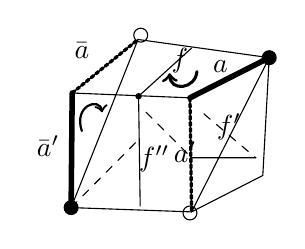
\begin{tikzpicture}[scale=.68,line cap=round]
\draw (0,0)--(2.25,-.08)--(3.58,.60)--(3.70,2.80)--(1.25,3.14)--(.02,2.14)--(2.22,2.05)--(2.25,-.08);
\draw[line width=2pt] (0,0)--(.02,2.14) (2.22,2.05)--(3.70,2.80);
\draw[densely dotted,line width=1.2pt] (.02,2.14)--(1.25,3.14) (2.22,2.05)--(2.25,-.08);
\draw (0,0)--(1.25,3.14) (2.25,-.08)--(3.70,2.80) (1.29,.03)--(1.26,2.08)--(2.25,2.98) (2.25,.93)--(3.45,.93);
\draw[dashed] (0,0)--(1.25,1.26) (1.40,1.78)--(2.25,.93) (2.48,1.75)--(3.45,.93);
\fill (0,0) circle (.14) (3.70,2.80) circle (.14) (1.26,2.08) circle (.06);
\draw (1.30,3.22) circle (.13) (2.22,-.10) circle (.13);
\draw[->,line width=1.1pt] (2.35,2.54) .. controls (2.32,2.21) and (1.85,2.16) .. (1.84,2.51);
\draw[->,thick] (.20,1.43) .. controls (.04,1.91) and (.53,2.07) .. (.58,1.78);
\node at (.20,2.93) {$\bar a$};\node at (-.43,1.14) {$\bar a'$};\node at (2.79,2.64) {$a$};
\node at (2.03,2.75) {$f$};\node at (1.55,.91) {$f''$};\node at (2.13,1.04) {$a'$};\node at (2.95,1.50) {$f'$};
\end{tikzpicture}}

\[
 \Sigma_a+\Sigma_{\bar a'}=\Sigma_{a'}+\Sigma_{\bar a}
\]

\[
 \begin{aligned}
 & &\tau_f+\tau_{f'}&=\Sigma_a & \tau_{\tilde f}+\tau_{\tilde f'}&=\Sigma_{\tilde a}=\Sigma_a\\
 &\unsure{4|7}\cdot3\cdot2=24=48/2\qquad &\tau_f\tau_{f'}&=\Pi_a & \tau_{\tilde f}\tau_{\tilde f'}&=\deleted{\unsure{\Pi}}\Pi_{\tilde a}=\Pi_a
 \end{aligned}
\]

donc $\{\tau_f,\tau_{f'}\}=\{\tau_{\tilde f},\tau_{\tilde f'}\}$

\figure{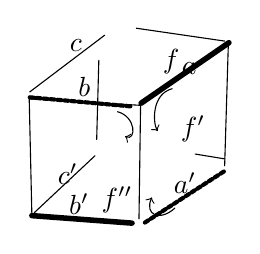
\begin{tikzpicture}[scale=.68,line cap=round]
\draw (0,.05)--(-.05,2.24)--(2.03,2.12)--(2,0) (2.02,2.12)--(3.67,3.30)--(3.60,.99) (3.6,3.32)--(1.95,3.56) (-.04,2.37)--(1.36,3.43);
\draw (.05,.12)--(1.18,1.18) (1.21,1.48)--(1.25,2.96) (3.05,1.21)--(3.60,1.12);
\draw[line width=2pt] (0,.06)--(1.87,-.08) (2.04,2.16)--(3.68,3.29);
\draw[densely dotted,line width=1.5pt] (-.04,2.27)--(1.85,2.10) (2.11,-.07)--(3.61,.90);
\draw[->] (1.60,2.0) .. controls (1.95,1.91) and (1.95,1.45) .. (1.74,1.54);
\draw[->] (2.62,2.43) .. controls (2.23,2.33) and (2.26,1.78) .. (2.35,1.64);
\draw[->] (2.67,.20) .. controls (2.38,-.06) and (2.1,.08) .. (2.24,.40);
\node at (.82,3.24) {$c$};\node at (.98,2.47) {$b$};\node at (2.60,2.94) {$f$};\node at (2.94,2.80) {$a$};
\node at (3.01,1.69) {$f'$};\node at (.67,.83) {$c'$};\node at (.88,.28) {$b'$};\node at (1.59,.35) {$f''$};\node at (2.86,.66) {$a'$};
\end{tikzpicture}}

\[
 \begin{aligned}
 \tau_f-\tau_{f''} &\unsure{=}\Sigma_a-\Sigma_{a'}=\Sigma_b-\Sigma_{b'} & \quad&\text{donc}\\
 \Sigma_a+\Sigma_{b'}&=\Sigma_b\unsure{-|+}\Sigma_{a'} &&
 \left\{\begin{aligned}\tau_f&=\tau_{\tilde f}\quad\text{\textcircled{ou}}\\
 \tau_f&=\tau_{\tilde f'}\end{aligned}\right.
 \end{aligned}
\]

\[
 \begin{aligned}
 \Sigma_a-\Sigma_{a'}&=\Sigma_c-\Sigma_{c'}\\
 \Sigma_a+\Sigma_{c'}&=\unsure{\Sigma_a|\Sigma_c}\unsure{-|+}\Sigma_c
 \end{aligned}
\]

$\Sigma_a$ ne dépend que de la direction de $a$ donc il \uline{n'y a que trois} \uline{valeurs} de $\Sigma_a$

de \unsure{=|même} il n'y a que trois valeurs de $\Pi_a$

\figure{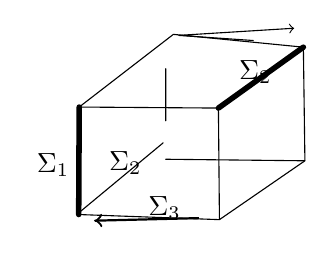
\begin{tikzpicture}[scale=.65,line cap=round]
\draw (0,0)--(2.75,-.10)--(4.42,1.05)--(4.39,3.27)--(1.85,3.52)--(.01,2.10)--(2.73,2.08)--(2.75,-.10);
\draw (.01,.04)--(1.65,1.40) (1.7,1.08)--(4.42,1.05) (1.70,1.83)--(1.70,2.85);
\draw[line width=2pt] (0,.0)--(.01,2.10) (2.73,2.08)--(4.39,3.27);
\draw[->,thick] (.32,-.12)--(2.35,-.07)--(.32,-.12);
\draw[->] (3.41,3.40)--(1.95,3.50)--(4.21,3.64);
\node at (-.50,.96) {$\Sigma_1$};\node at (.91,1.00) {$\Sigma_2$};\node at (1.68,.12) {$\Sigma_3$};\node at (3.45,2.79) {$\Sigma_2$};
\end{tikzpicture}}

$12$ relations de la forme $\Sigma_a+\Sigma_{a'}=\Sigma_b+\Sigma_{b'}$, \deleted{pour $\Sigma_a$ fixé} via opérations du groupe symétrique $\unsure{\mathfrak S|\mathscr S}_4$, elles se déduisent \unsure{l'une de l'autre|les unes des autres}
